\chapter{Solución Propuesta}

La solución propuesta parte del diseño de una arquitectura modular que integra
varios subsistemas electrónicos en una estación de control ESD. Cada subsistema
cumple una función específica: verificar la pulsera antiestática, identificar al
usuario, presentar el resultado de la prueba y almacenar los registros para
generar reportes. Además, los registros incorporan la temperatura y la humedad
relativa como información complementaria.

En este documento, el término sistema comprende la solución completa, incluidos
el hardware, el software y la comunicación entre los subsistemas, mientras que
estación se refiere al equipo físico con el que interactúa el usuario.

Desde el punto de vista operativo, antes de trabajar en el laboratorio, cada
usuario deberá identificarse y realizar la prueba de la pulsera antiestática. La
estación registrará el resultado antes de que el usuario manipule dispositivos
electrónicos o inicie actividades dentro del área de trabajo. Este procedimiento
se muestra en la Figura~\ref{fig:flujo_sistema}
\cite{ESDAFundamentalsPart3}.

\begin{figure}[H]
    \centering
    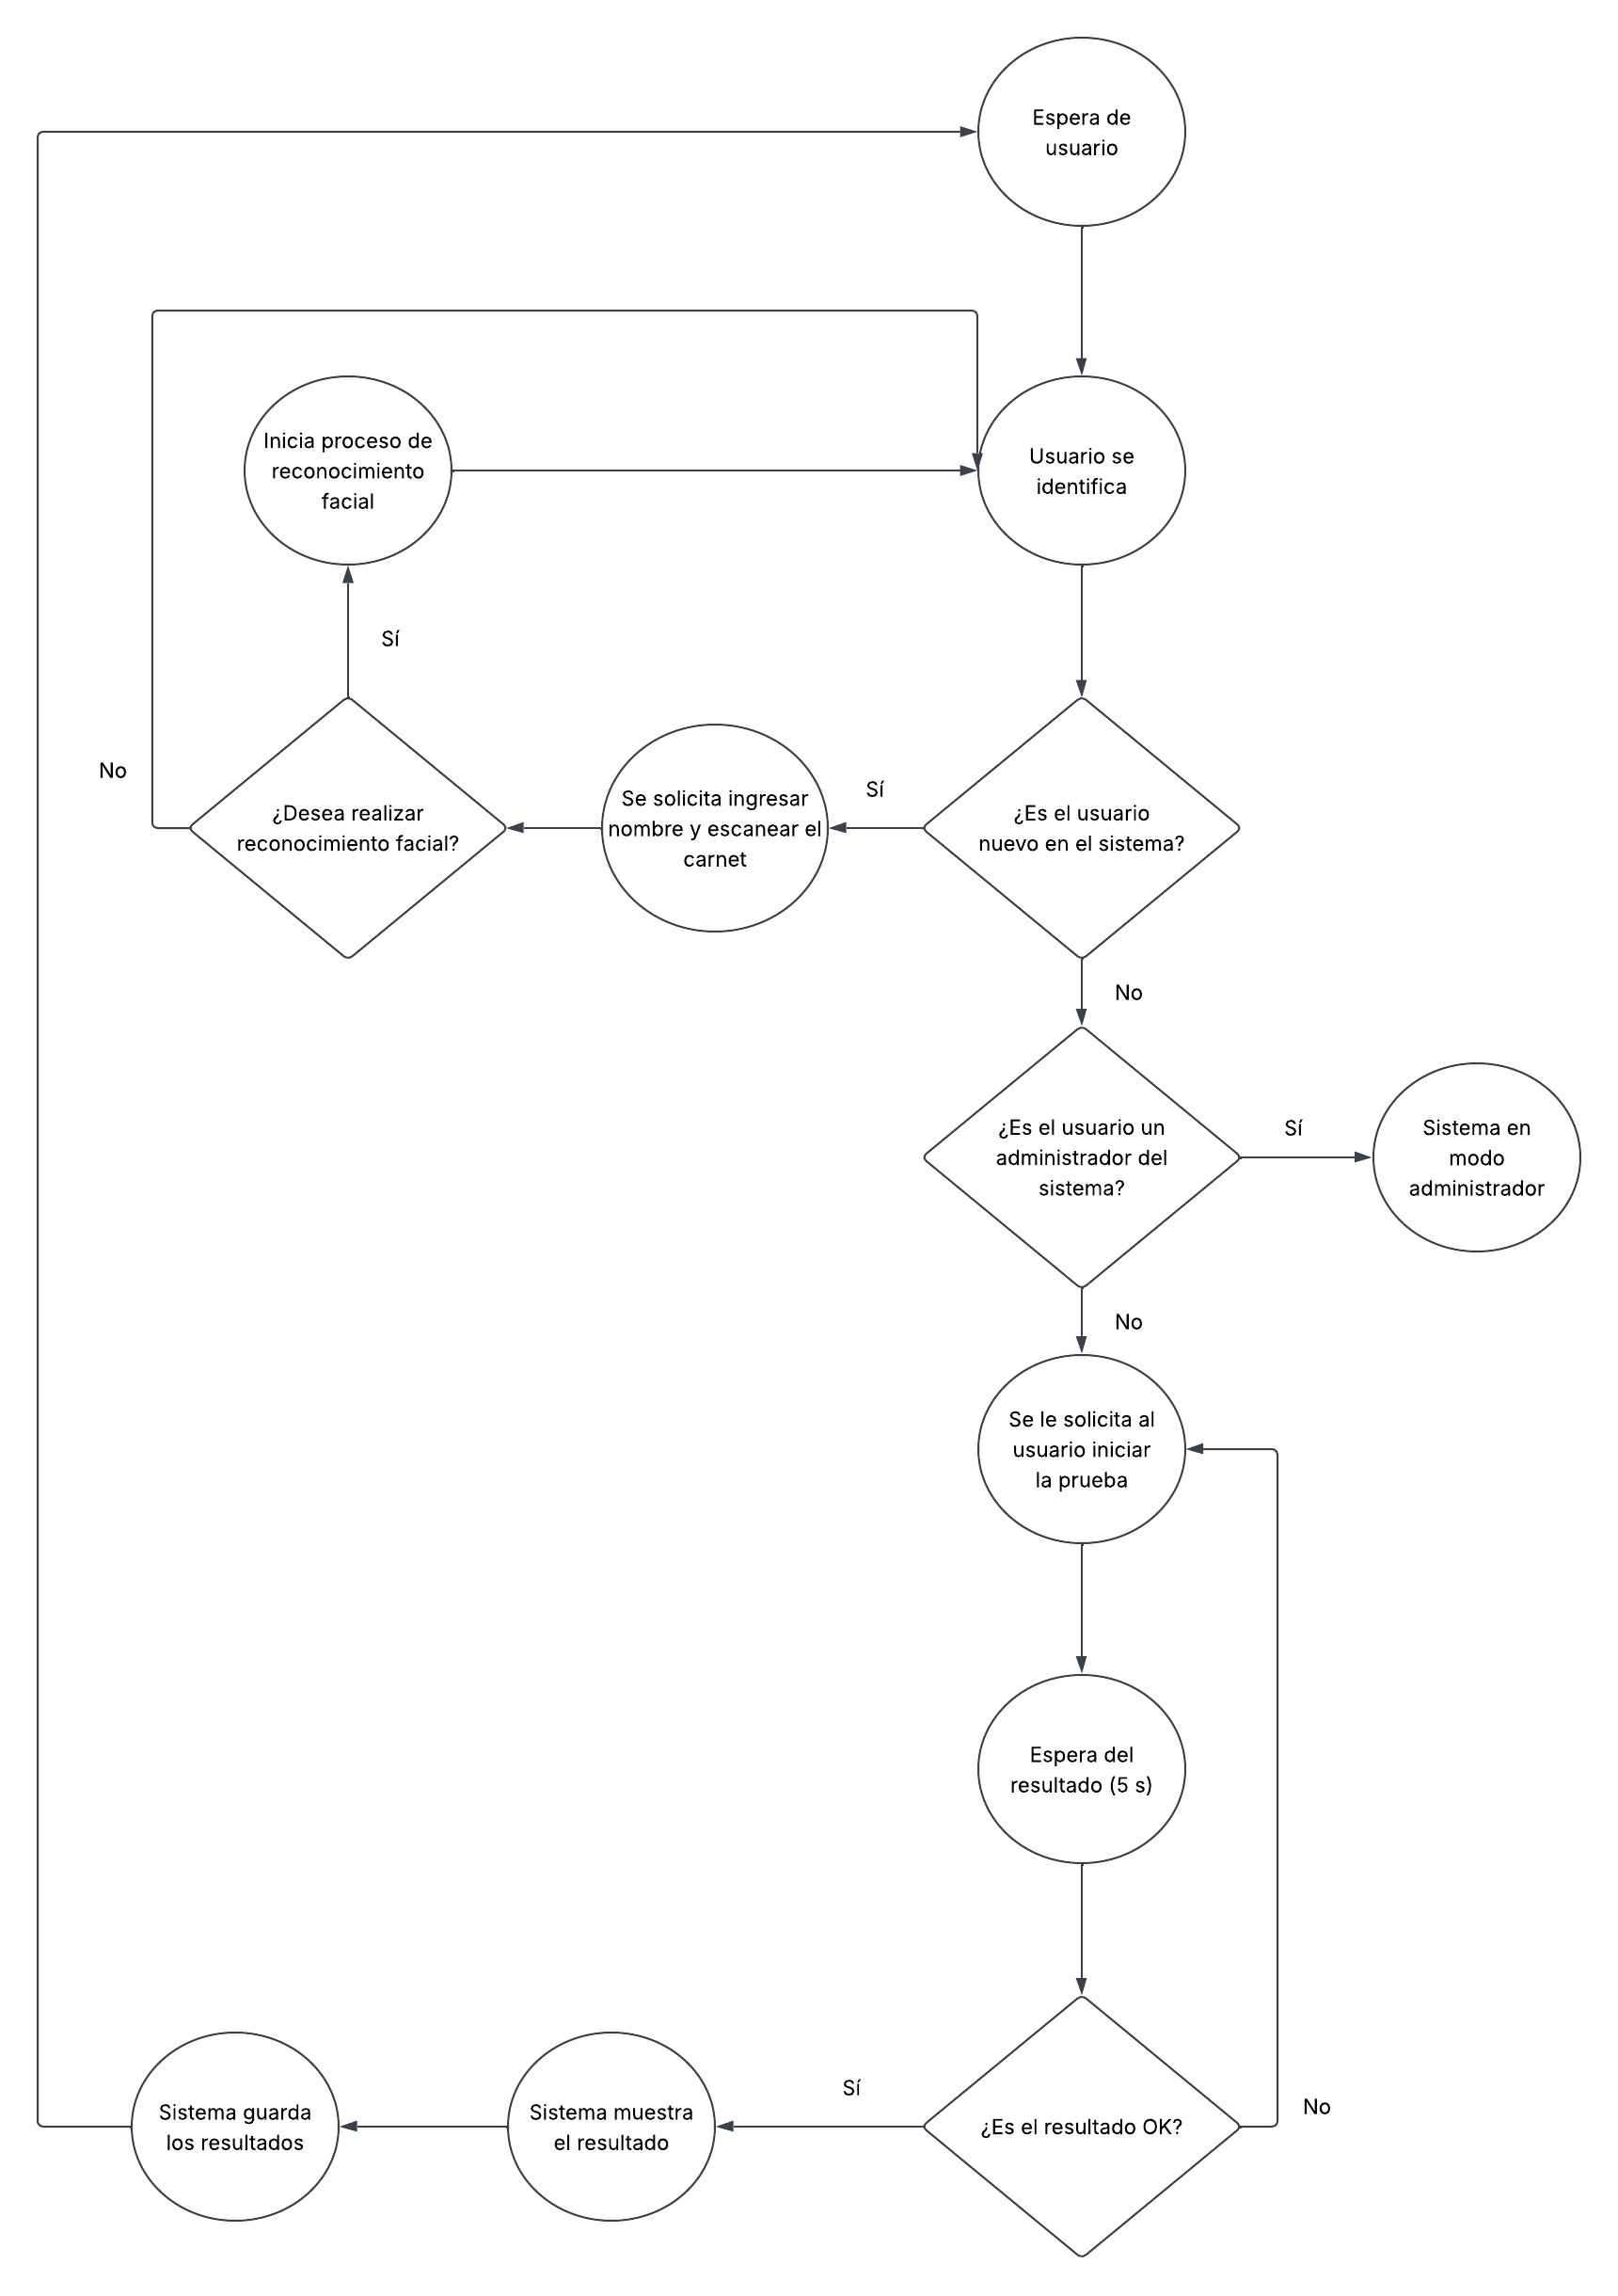
\includegraphics[width=0.7\textwidth]{pics/SP_22.png}
    \caption{Flujo de prueba del sistema propuesto, fuente:
    elaboración propia.}
    \label{fig:flujo_sistema}
\end{figure}

Para implementar esta arquitectura y su flujo de operación, los componentes se
seleccionaron considerando su compatibilidad eléctrica, interfaces de
comunicación, disponibilidad comercial, costo, consumo de potencia y facilidad de
integración en el prototipo. También se consideró la modularidad, de manera que
la modificación de un subsistema no obligue a rediseñar completamente la
estación. A continuación se describen los componentes seleccionados y las
decisiones de ingeniería asociadas.

\section{Sistema de verificación ESD}

El subsistema de verificación ESD requiere un dispositivo capaz de evaluar el
estado de la pulsera antiestática del usuario siguiendo los estándares y manteniendo 
la medición dentro de una precisión adecuada, también debe entregar una indicación clara
del resultado de la prueba. Además, debido al alcance del proyecto, se requiere
una solución que permita reducir la complejidad asociada al diseño de circuitos
propios para medición de alta resistencia, de forma que el desarrollo pueda
centrarse en la integración, la trazabilidad y la gestión de registros.

A partir de estos criterios, se propone utilizar el probador HZR 171 como
subsistema principal para la evaluación de la pulsera antiestática del usuario.
Este dispositivo permite verificar si la resistencia eléctrica asociada al
sistema usuario-pulsera se encuentra dentro de un rango aceptable de operación.
De acuerdo con la información del fabricante, el dispositivo es capaz de medir
resistencias entre $800~\mathrm{k}\Omega$ y $10~\mathrm{M}\Omega$ con una
precisión de $\pm 10~\%$, lo cual lo convierte en una alternativa adecuada para
la verificación de pulseras antiestáticas dentro del alcance del proyecto
\cite{hzr171_oficial}.

La selección de este probador también se justifica porque permite utilizar una
plataforma comercial existente para la etapa de verificación ESD, evitando que
el prototipo dependa de un circuito de medición desarrollado desde cero \cite{keithley_lowlevel}. Esto
reduce riesgos técnicos relacionados con mediciones de alta impedancia,
calibración, seguridad eléctrica y repetibilidad de la prueba
\cite{keithley_lowlevel,S1_1_ANSI}.

Sin embargo, no se plantea su uso como probador para sistemas de tobilleras o
calzado ESD, debido a que estos elementos pueden requerir rangos de evaluación
y criterios de aceptación diferentes a los soportados por el dispositivo
seleccionado. Por esta razón, el alcance de la solución se limita a la
verificación de pulseras antiestáticas
\cite{IEC61340_4_6,STM97_ANSI}.

\begin{figure}[H]
    \centering
    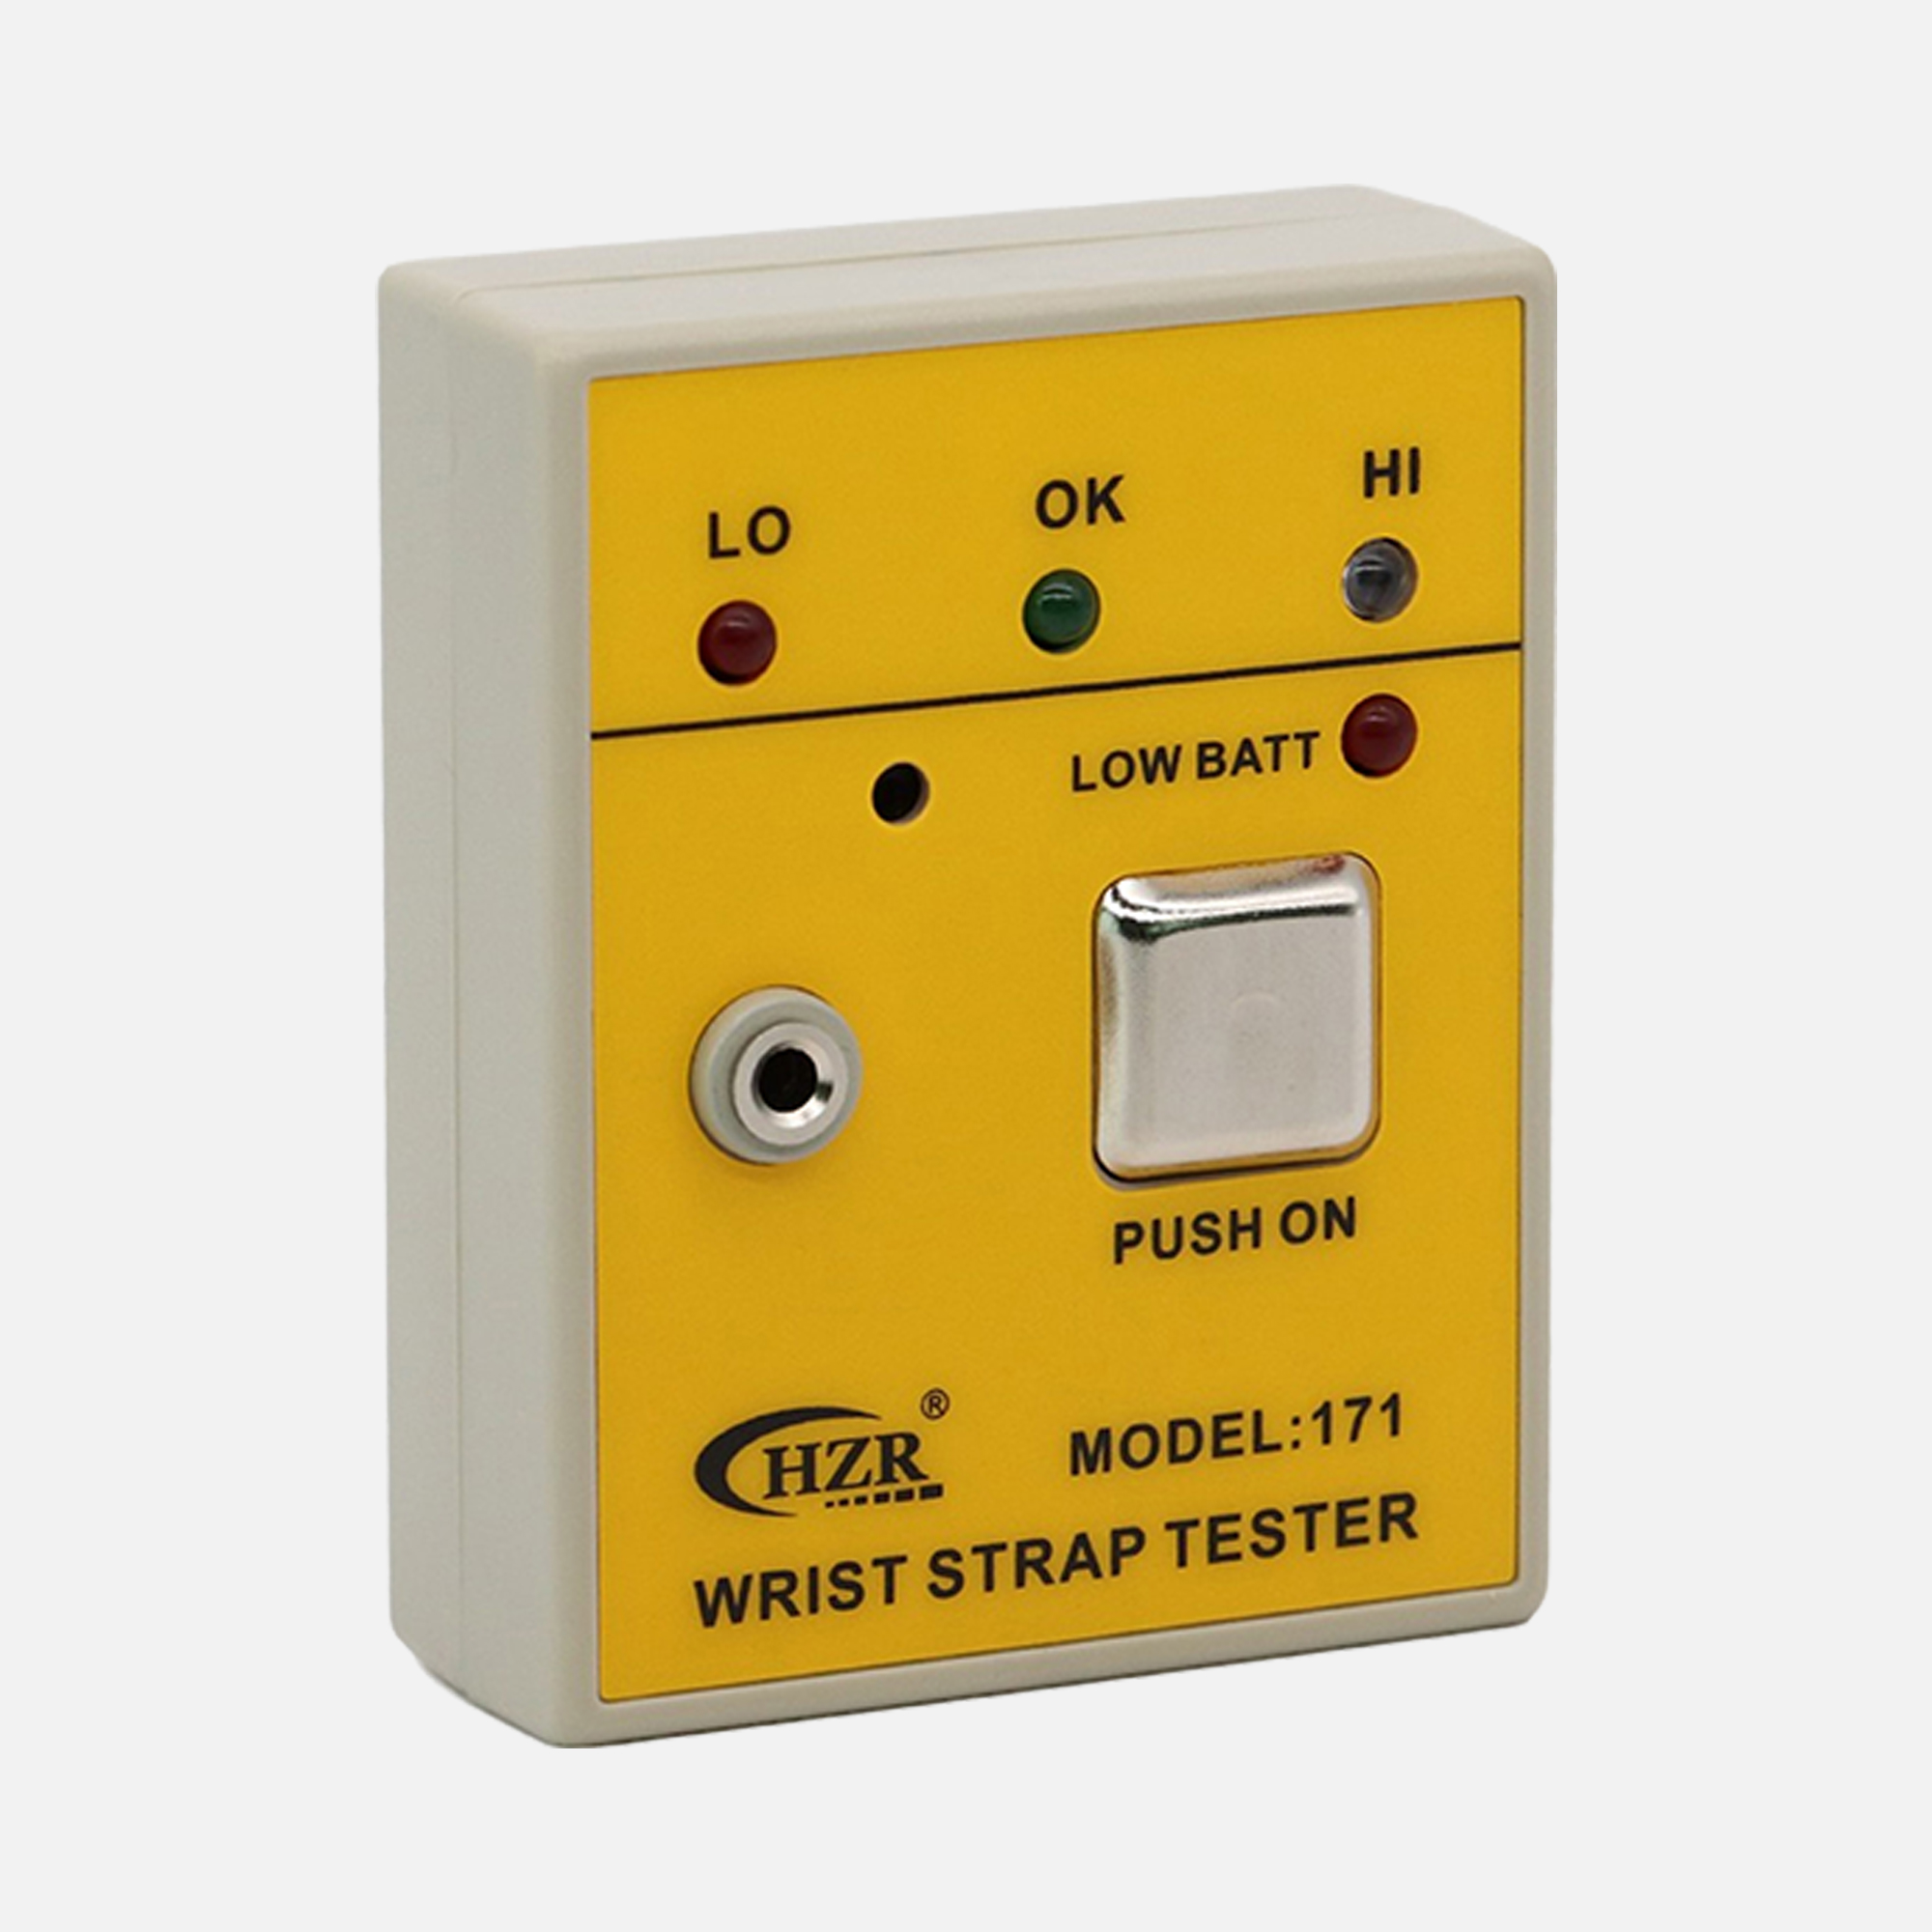
\includegraphics[width=0.45\textwidth]{pics/SP_06.jpg}
    \caption{Probador de pulseras antiestáticas HZR 171, fuente de imagen:
    \cite{hzr171_oficial}.}
    \label{fig:hzr171_tester}
\end{figure}

La tarjeta electrónica del HZR 171 será utilizada como base del subsistema de
verificación ESD. Para su integración con el sistema general, se emplearán las
señales digitales $LO$, $OK$ y $HI$, las cuales permiten identificar si la
resistencia medida se encuentra por debajo del rango aceptable, dentro del rango
correcto o por encima del límite establecido \cite{hzr171_oficial}. Estas señales serán leídas por el
controlador correspondiente mediante entradas digitales.

Además, debido a que el dispositivo requiere una alimentación de
$9~\mathrm{VDC}$ \cite{hzr171_oficial}, dicha tensión será generada a partir del
sistema de alimentación principal del prototipo, tal como se explica más
adelante en este capítulo.

Para la lectura de las señales digitales del probador se plantea utilizar,
inicialmente, un divisor resistivo como conversor de nivel lógico. Esta etapa es
necesaria porque los GPIO del ESP32 pertenecen al dominio de
$3.3~\mathrm{VDC}$ \cite{esp32wroom}, mientras que la tensión de las salidas del
HZR-171 todavía debe caracterizarse. Por tanto, las señales no se conectarán
directamente al microcontrolador antes de medir su tensión en estado alto y
en estado bajo.

\begin{figure}[H]
    \centering
    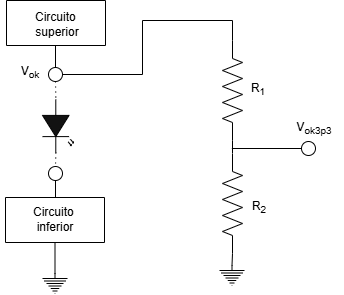
\includegraphics[width=0.45\textwidth]{pics/SP_19.png}
    \caption{Conversor de nivel de tensión a 3.3 VDC, fuente de imagen:
    elaboración propia.}
    \label{fig:conversor_nivel_tension}
\end{figure}

Para una salida positiva $V_{\mathrm{HZR}}$, el divisor de la
Figura~\ref{fig:conversor_nivel_tension} produce la tensión

\begin{equation}
    V_{\mathrm{GPIO}} =
    V_{\mathrm{HZR}}\frac{R_2}{R_1+R_2}.
    \label{eq:divisor_nivel_hzr}
\end{equation}

Los valores de $R_1$ y $R_2$ se definirán después de caracterizar las salidas
$LO$, $OK$ y $HI$. El diseño deberá garantizar que la máxima tensión aplicada
al GPIO no exceda el límite admitido por el ESP32 y, al mismo tiempo, que el
nivel reducido permanezca por encima de la tensión mínima reconocida como
estado lógico alto \cite{esp32wroom}. También se utilizaran valores de resistencias
en el rango de los kiloohmios para asegurar que la salia del probador no se verá
afectada por sobrecorriente.

\section{Sistema de identificación de usuarios}

El sistema de identificación de usuarios requiere mecanismos que permitan asociar
cada prueba ESD con una persona específica. Esta asociación es necesaria para
convertir una verificación local en un evento trazable, consultable y auditable \cite{ESDA1}.
Para ello, se plantea utilizar dos mecanismos complementarios: lectura de código
de barras y reconocimiento facial.

La lectura de código de barras se establece como el mecanismo principal de
identificación, ya que permite utilizar los gafetes empresariales existentes sin
modificar la infraestructura del laboratorio. Por su parte, el reconocimiento
facial se plantea como un mecanismo complementario, orientado a reforzar la
validación del usuario y evaluar una alternativa adicional de identificación
dentro del prototipo.

\subsection{Reconocimiento facial}

Para el subsistema de reconocimiento facial se requiere una plataforma compacta,
de bajo costo, con cámara integrada, capacidad de procesamiento embebido y
posibilidad de comunicación con el controlador principal. Estas características
son necesarias para separar la captura y el procesamiento básico de imagen del
resto del sistema, manteniendo una arquitectura modular.

A partir de estos criterios, se plantea utilizar el módulo Freenove ESP32-S3 CAM
para implementar el subsistema de reconocimiento facial. Este dispositivo
incorpora una cámara y un microcontrolador ESP32-S3, lo que permite ejecutar
algoritmos livianos de procesamiento de imagen y reconocimiento dentro de un
módulo compacto y de bajo costo \cite{esp32s3}.

La selección de este módulo se justifica porque integra en una sola placa los
elementos necesarios para capturar imágenes, procesarlas localmente y comunicar
el resultado al sistema principal. Además, al estar basado en la familia ESP32,
facilita la comunicación inalámbrica con otros microcontroladores del sistema y
mantiene coherencia con la arquitectura embebida propuesta
\cite{FreenoveESP32S3CAM}.

La función principal de este módulo será realizar el proceso de captura y
verificación facial. Posteriormente, el resultado de la identificación será
enviado al controlador principal para ser asociado con el resultado de la prueba
ESD y con el registro correspondiente.

Como base de software se utilizarán herramientas de visión artificial
proporcionadas por Espressif. El controlador \texttt{esp\_camera} realizará la
captura de las imágenes, mientras que los modelos y funciones basados en ESP-DL
ejecutarán la detección y el reconocimiento facial. Estas herramientas también
forman parte del ecosistema utilizado por ESP-WHO. Se considerarán inicialmente
un modelo cuantizado y una resolución moderada para reducir el uso de memoria y
el tiempo de respuesta \cite{ESPWHO,ESPDLGuide,ESP32Camera}.

El flujo propuesto para el código consiste en inicializar la cámara, la PSRAM,
el modelo y las identidades; capturar una imagen; localizar el rostro; obtener
su huella facial (\textit{face embedding}); compararla con los usuarios
registrados; y aplicar un umbral para producir el resultado. El módulo enviará
al controlador principal únicamente el identificador o estado obtenido, sin
transmitir la imagen completa. El ejemplo \textit{CameraWebServer} se utilizará
como referencia para la inicialización de la cámara y el manejo de los búferes
\cite{ArduinoCameraWebServer}.

La configuración final deberá determinarse experimentalmente. Se medirán las
detecciones correctas, falsas aceptaciones, falsos rechazos, tiempo de
inferencia y uso de RAM y PSRAM. Las pruebas incluirán cambios controlados de
iluminación, distancia, ángulo y movimiento, además de diferentes umbrales y
cantidades de identidades. Esto permitirá establecer las condiciones bajo las
cuales el reconocimiento es suficientemente confiable para utilizarse como
mecanismo complementario \cite{NISTFRTE11}.

\begin{figure}[H]
    \centering
    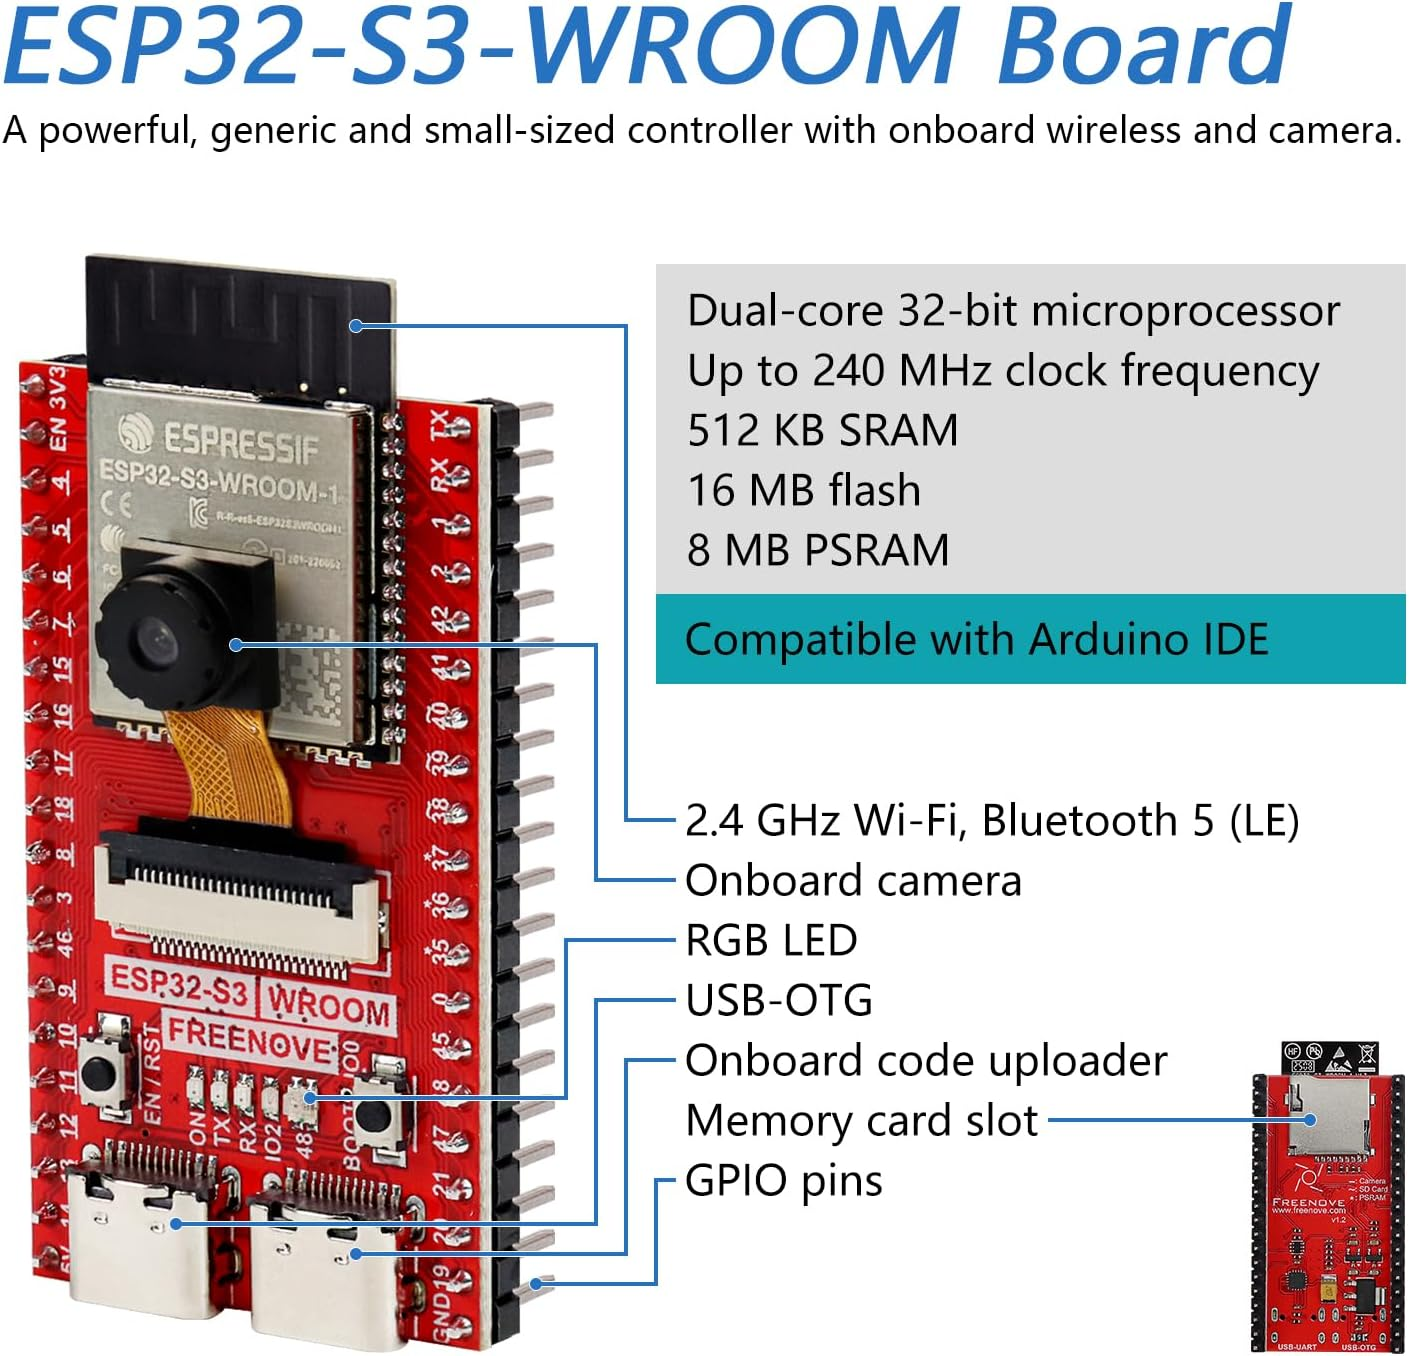
\includegraphics[width=0.45\textwidth]{pics/SP_07.jpg}
    \caption{Módulo Freenove ESP32-S3 CAM utilizado para reconocimiento facial,
    fuente de imagen: \cite{FreenoveESP32S3CAM}.}
    \label{fig:esp32s3_cam_freenove}
\end{figure}

\subsection{Lectura de código de barras}

Para la identificación mediante código de barras, el sistema requiere un lector
compacto, compatible con códigos 1D y 2D, con una interfaz de comunicación
sencilla y capaz de operar bajo las condiciones de iluminación del laboratorio.
También se requiere que el lector pueda integrarse con un microcontrolador
embebido sin agregar una complejidad significativa al sistema.

A partir de estos criterios, se propone utilizar el módulo GM67, el cual soporta
comunicación UART, facilitando su integración con el microcontrolador secundario
ESP32-WROOM. La selección de este módulo responde a tres criterios principales:
compatibilidad con códigos 1D y 2D, facilidad de comunicación mediante interfaz
serial y operación bajo un amplio rango de iluminación \cite{GM67}.

De acuerdo con la documentación técnica del dispositivo, el GM67 puede operar
bajo condiciones de iluminación entre $0$ y $100000~\mathrm{lux}$, lo que reduce
la dependencia de la iluminación ambiental del laboratorio \cite{GM67}. 
Esta característica permite utilizar los gafetes
empresariales como mecanismo de identificación sin modificar la infraestructura
existente.

Por tanto, el módulo GM67 se considera una alternativa adecuada para el
subsistema de identificación principal, ya que permite leer el identificador del
usuario de forma directa y comunicarlo al controlador principal por medio del
ESP32-WROOM, para asociarlo con el resultado de la prueba ESD.

\begin{figure}[H]
    \centering
    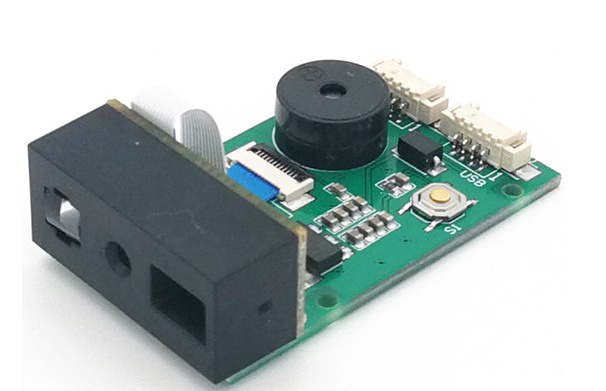
\includegraphics[width=0.58\textwidth]{pics/SP_23.jpg}
    \caption{Módulo lector de código de barras GM67, fuente de imagen:
    \cite{GM67}.}
    \label{fig:gm67_barcode}
\end{figure}

\section{Registro complementario de variables ambientales}

Como función complementaria, el sistema registrará la temperatura y la humedad
relativa asociadas a cada prueba ESD. Estos datos permitirán documentar las
condiciones del entorno, pero no determinarán el resultado de la prueba ni
constituirán el eje principal de la solución. Para adquirirlos se requiere un
sensor compatible con sistemas embebidos y de baja complejidad de integración.

A partir de estos criterios, se propone utilizar el sensor SHT31-D, dispositivo
capaz de medir temperatura y humedad relativa de forma simultánea. El sensor
posee un rango de medición de humedad relativa entre $0$ y $100~\%$ HR con una
precisión de $\pm 2~\%$ HR, mientras que para la temperatura ofrece un rango
entre $-40~^\circ\mathrm{C}$ y $125~^\circ\mathrm{C}$ con una precisión de
$\pm 0.2~^\circ\mathrm{C}$ \cite{sht31d_datasheet}.

Estas características permiten incorporar el contexto ambiental a los registros
sin agregar una complejidad significativa al sistema. La humedad relativa es una
variable relevante en entornos de control electrostático, pues condiciones secas
pueden favorecer la acumulación de carga \cite{ESDA1}.

El módulo utiliza comunicación I2C, protocolo ampliamente soportado por
microcontroladores modernos y adecuado para integrar sensores de baja velocidad
en sistemas embebidos \cite{ti_basic_guide_i2c}. Además, el
sensor se encuentra disponible en tarjetas PCB con pines de comunicación I2C, lo
cual facilita su integración en el prototipo sin requerir un proceso de soldadura
SMD.

\begin{figure}[H]
    \centering
    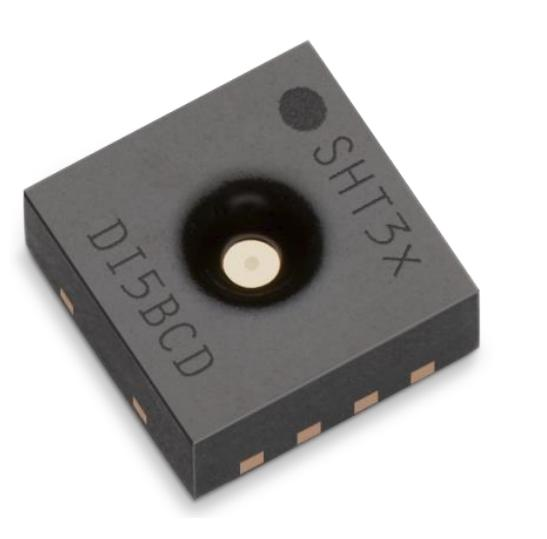
\includegraphics[width=0.45\textwidth]{pics/SP_10.jpg}
    \caption{Sensor de humedad relativa y temperatura SHT31-D, fuente:
    \cite{sht31d_datasheet}.}
    \label{fig:sht31_sensor}
\end{figure}

\section{Sistema de procesamiento, interfaz y almacenamiento}

\subsection{Controlador principal e interfaz gráfica}

El sistema requiere un controlador principal capaz de coordinar los subsistemas
del prototipo, ejecutar la interfaz gráfica, gestionar la interacción con el
usuario y administrar el almacenamiento local de registros. Además, se requiere
una pantalla táctil que permita guiar al usuario durante el flujo de prueba y
mostrar el resultado de la verificación ESD de forma clara.

A partir de estos criterios, se propone utilizar el HMI ELECROW ESP32 de
$7$ pulgadas. Este módulo incorpora una pantalla táctil, un microcontrolador
ESP32-S3, DAC para reproducción de sonido, múltiples puertos de comunicación y
soporte para memorias microSD \cite{ElecrowESP32HMIManual}.

La selección de este HMI se justifica porque integra en una sola plataforma el
controlador principal, la interfaz gráfica táctil y recursos de almacenamiento.
Esto permite reducir la cantidad de módulos externos, simplificar el cableado
del prototipo y centralizar la operación del sistema. Además, al estar basado en
ESP32-S3, mantiene compatibilidad con herramientas de desarrollo para sistemas
embebidos y con protocolos de comunicación utilizados por otros módulos del
prototipo \cite{esp32s3}.

El microcontrolador integrado en el HMI será utilizado como controlador principal
del sistema. Este dispositivo interactuará con todos los subsistemas, ya sea de
forma directa o indirecta. En el caso de la comunicación directa, el HMI se
conectará con el sensor ambiental y el parlante mediante los puertos de
comunicación disponibles. De forma indirecta, obtendrá los datos del probador
HZR 171 y del lector de códigos de barras mediante el microcontrolador
secundario ESP32-WROOM. Asimismo, el controlador principal se comunicará con el
módulo ESP32-S3 CAM, encargado de capturar las imágenes, ejecutar localmente el
reconocimiento facial y enviar únicamente el resultado de la identificación al
HMI. 

La comunicación entre el HMI, el microcontrolador secundario ESP32-WROOM y el
módulo de reconocimiento facial ESP32-S3 CAM se realizará mediante ESP-NOW. Este
protocolo permite comunicación directa entre dispositivos compatibles sin
depender de un enrutador o de una red institucional y admite múltiples
dispositivos emparejados \cite{espressif_espnow}. Esta característica favorece
una arquitectura modular y evita que el funcionamiento básico de la estación
dependa de la infraestructura inalámbrica del laboratorio.

En la Figura~\ref{fig:pin_out_hmi_elecrow_esp32} se muestra la distribución de
los puertos de entrada y salida del HMI ELECROW ESP32.

\begin{figure}[H]
    \centering
    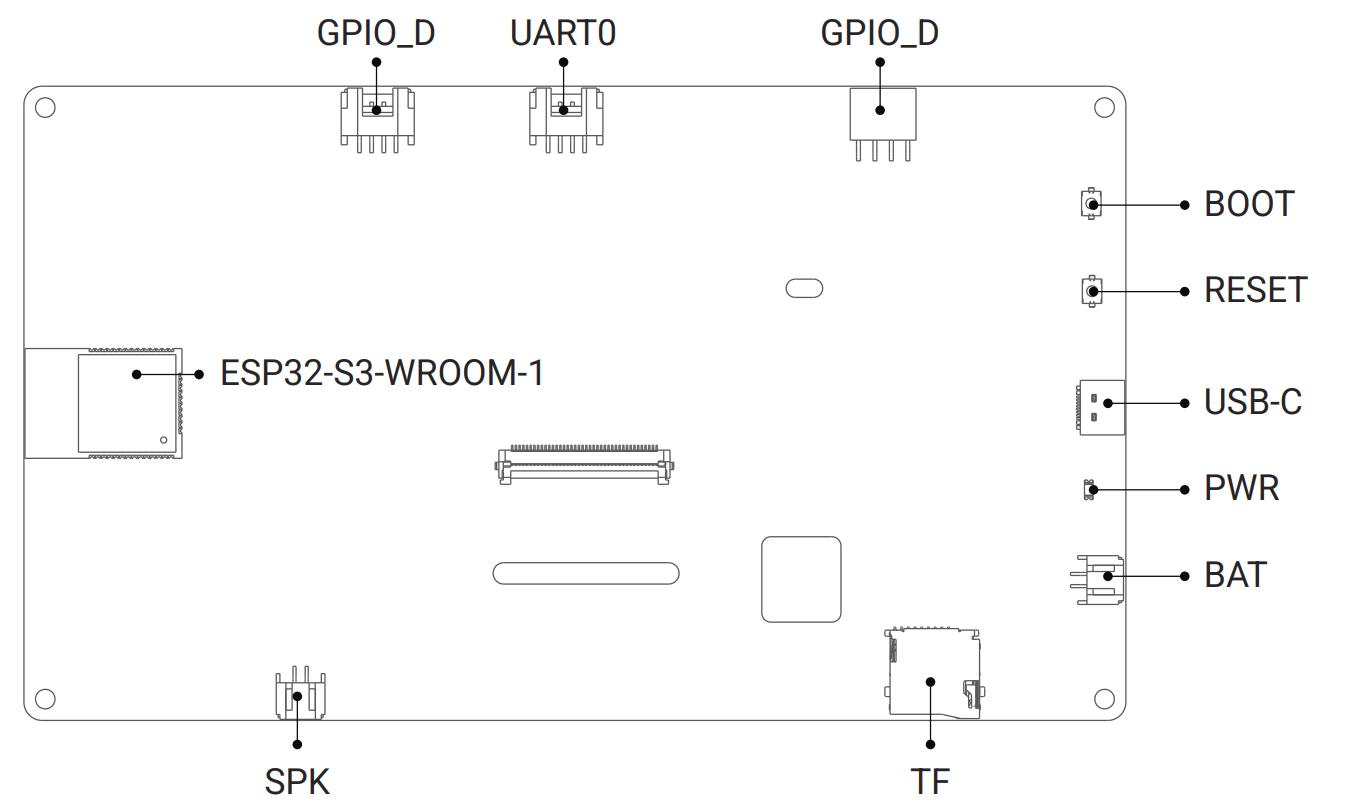
\includegraphics[width=0.70\textwidth]{pics/SP_24.jpg}
    \caption{Diagrama de puertos del HMI ELECROW ESP32 de $7$ pulgadas, fuente:
    \cite{elecrow_esp32_wiki}.}
    \label{fig:pin_out_hmi_elecrow_esp32}
\end{figure}

La interfaz gráfica permitirá guiar al usuario durante el proceso de prueba,
mostrar el estado del sistema, indicar el resultado de la verificación ESD y
facilitar la consulta de registros. Además, el sistema de audio permitirá
generar retroalimentación sonora para mejorar la interacción con el usuario.

\begin{figure}[H]
    \centering
    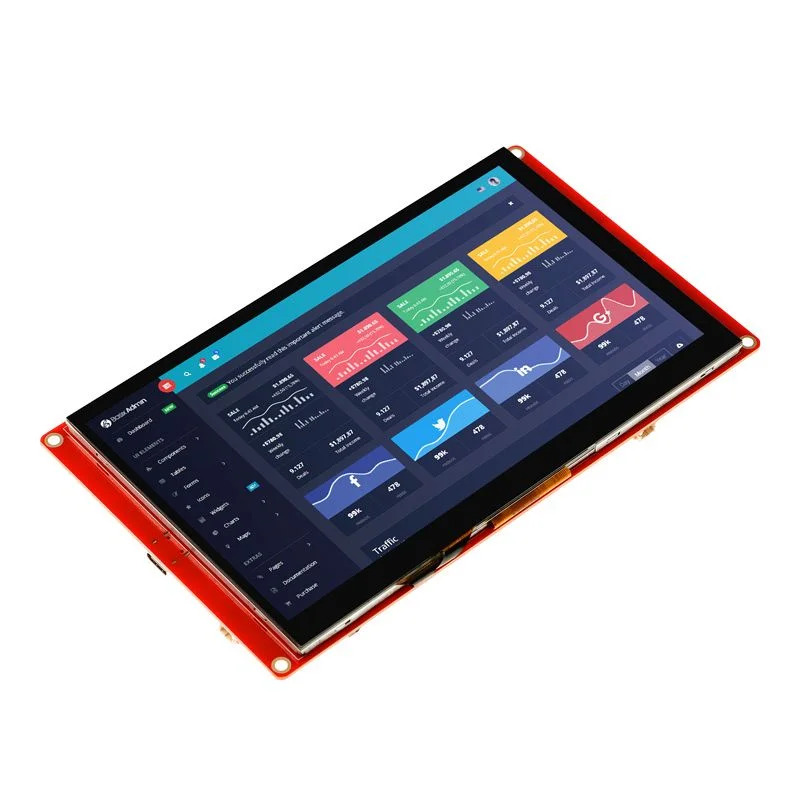
\includegraphics[width=0.65\textwidth]{pics/SP_12.jpg}
    \caption{HMI ELECROW ESP32 de $7$ pulgadas, fuente:
    \cite{elecrow_esp32_wiki}.}
    \label{fig:hmi_elecrow_esp32}
\end{figure}

\subsection{Controlador secundario para integración del probador ESD y el lector GM67}

Para integrar el probador HZR 171 y el lector GM67 con el resto del sistema se
requiere un controlador secundario. Este dispositivo leerá las señales digitales
del probador ESD y se comunicará con el GM67 mediante UART para recibir el código
de identificación del usuario. Posteriormente, enviará ambos datos al controlador
principal mediante ESP-NOW. Esta separación permite mantener el HMI como unidad
principal de interfaz y almacenamiento, mientras que el microcontrolador
secundario se encarga de la interacción directa con ambos dispositivos.

A partir de estos criterios, se plantea utilizar un microcontrolador ESP32-WROOM
como controlador secundario. Este dispositivo posee entradas y salidas digitales,
interfaces UART, capacidad de comunicación inalámbrica y compatibilidad con
ESP-NOW, lo que facilita su integración con el probador, el lector GM67 y el HMI
\cite{esp32wroom}.

\begin{figure}[H]
    \centering
    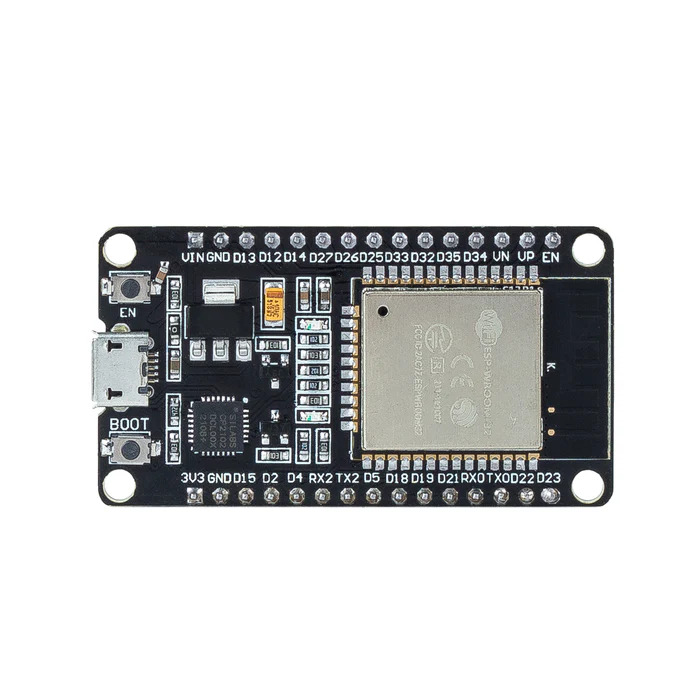
\includegraphics[width=0.55\textwidth]{pics/SP_25.jpg}
    \caption{ESP32 WROOM, fuente:
    \cite{sunfounder_esp_wroom_32_devboard}.}
    \label{fig:esp32_wroom_secundario}
\end{figure}

La utilización de un controlador secundario mejora la modularidad al separar la
adquisición del probador ESD del procesamiento de la interfaz gráfica. De esta
forma, una modificación del circuito de acondicionamiento o del probador podría
realizarse sin alterar de manera significativa la lógica principal del HMI.
Además, el ESP32-WROOM dispone de GPIO e interfaces de comunicación que pueden
reservarse para ampliaciones futuras \cite{esp32wroom}. Esta capacidad de
expansión se considerará solamente después de asignar los pines requeridos por
las funciones actuales y verificar que no correspondan a pines de arranque o
con funciones restringidas.

\subsection{Almacenamiento local y generación de reportes}

El sistema requiere almacenar localmente los eventos generados durante la
operación del prototipo. Cada registro debe incluir el nombre y el identificador
del usuario, la fecha, la hora, el resultado de la prueba ESD, el estado de
identificación y las variables ambientales asociadas. Para cumplir con este requerimiento, se
utilizará almacenamiento local mediante una memoria microSD integrada en el
ESP32-S3 HMI \cite{ElecrowESP32HMIManual}.

La selección de almacenamiento microSD se justifica porque permite guardar
archivos de forma local, operar sin conexión permanente a internet y generar
reportes históricos en formatos simples. Además, el uso de archivos CSV resulta
adecuado para el prototipo porque es un formato ligero, fácil de generar desde
un sistema embebido y compatible con herramientas comunes de análisis de datos
\cite{RFC4180}.

Cada registro incluirá, como mínimo, el nombre y el identificador del usuario,
la fecha, la hora, el resultado ESD, el método de identificación, la temperatura
y la humedad relativa. El
sistema verificará el resultado de la escritura antes de informar que el ciclo
fue registrado. Si ocurre una pérdida de comunicación, un dato obligatorio está
ausente o la escritura falla, el evento se marcará como incompleto y no deberá
contabilizarse como una prueba trazable. Este criterio se relaciona directamente
con la hipótesis, que establece una proporción mínima de 95~\% de registros
completos.

El almacenamiento local permite que el prototipo opere sin depender de
plataformas externas, servicios en la nube o bases de datos corporativas. Esto
mantiene el alcance del proyecto dentro de una validación académica controlada y
reduce la exposición de datos personales durante las pruebas de operación.

\subsubsection{Referencia temporal mediante un módulo RTC}

La trazabilidad de las verificaciones ESD requiere asociar cada registro con la
fecha y la hora en que se ejecutó la prueba. Debido a que el prototipo puede
desconectarse de su alimentación y no dependerá de una conexión
permanente a internet, se propone utilizar un módulo de reloj de tiempo real
(RTC, por sus siglas en inglés) DS3231 con alimentación de respaldo.

El DS3231 se conectará mediante I2C al controlador secundario ESP32-WROOM. Al
detectar el resultado de una prueba, este controlador obtendrá la fecha y la
hora del módulo y las enviará mediante ESP-NOW, junto con el identificador del
usuario y el resultado ESD, al controlador principal para generar el registro
correspondiente.

La selección del DS3231 se fundamenta en su interfaz I2C, su compatibilidad con
sistemas de $3.3$~V y su oscilador compensado por temperatura, que reduce la
desviación de la hora ante cambios de temperatura. Además, su alimentación de
respaldo permite conservar la referencia temporal cuando el prototipo se
desconecta \cite{AnalogDevices_DS3231}.

\section{Sistema de alimentación eléctrica}

El prototipo requiere dos niveles de alimentación para su funcionamiento: una
línea principal de $5~\mathrm{VDC}$ para la mayoría de los subsistemas y una
salida de $9~\mathrm{VDC}$, generada a partir de dicha línea, para alimentar el
probador HZR 171. Por lo tanto, el sistema de alimentación debe ser compatible
con los módulos seleccionados y mantener una arquitectura compacta.

Como entrada principal se utilizará un módulo comercial USB-C PD configurado
para entregar una línea de $5~\mathrm{V}$. Este módulo recibirá la energía desde
un adaptador externo compatible y evitará diseñar dentro del alcance del
proyecto un circuito propio para gestionar la entrada de alimentación USB-C PD
\cite{usbif_usb_power_delivery}.

A partir de la salida del módulo se realizará una distribución independiente
de la línea de $5~\mathrm{V}$. Una rama se conectará a los pines de alimentación
de $5~\mathrm{V}$ del ESP32-WROOM y otra al módulo ESP32-S3 CAM. Para el HMI, una
rama terminará en un conector USB-C y se conectará mediante un cable al puerto
USB-C hembra de la pantalla. De esta forma, el HMI no se utilizará como fuente
para los demás subsistemas, sino como una carga adicional de la línea principal.
La misma línea alimentará el convertidor elevador encargado de generar los
$9~\mathrm{V}$ requeridos por el probador HZR 171.

Después del módulo USB-C PD se propone una etapa de protección en la línea de
$5~\mathrm{V}$,
mostrada en la Figura~\ref{fig:proteccion_picos}. El elemento en serie representa
un fusible para limitar condiciones de sobrecorriente. El diodo
conectado en paralelo representa un supresor TVS y el condensador representa la
reserva local de energía de la línea. Estos elementos cumplen funciones
diferentes: el fusible protege ante una corriente sostenida, el TVS desvía
transitorios breves y el condensador reduce variaciones de tensión causadas por
cambios rápidos de carga.

\begin{figure}[H]
    \centering
    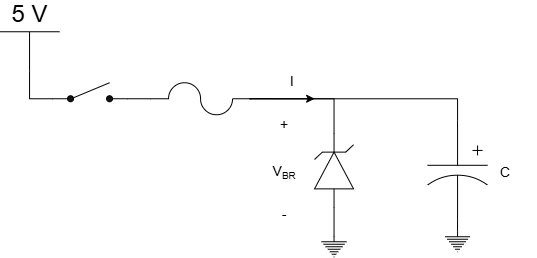
\includegraphics[width=0.65\textwidth]{pics/SP_26.png}
    \caption{Circuito de protección contra picos de tensión y sobrecorriente,
    fuente: elaboración propia.}
    \label{fig:proteccion_picos}
\end{figure}

La selección del TVS no dependerá únicamente de escoger una tensión de ruptura
ligeramente superior a $5~\mathrm{V}$. Se deberán considerar su tensión inversa
de trabajo, tensión de ruptura, tensión de sujeción y capacidad de disipación.
Durante la operación nominal el dispositivo no deberá conducir, mientras que
durante un transitorio su tensión de sujeción deberá permanecer dentro del
límite tolerado por los circuitos conectados. Estos parámetros corresponden a
los criterios recomendados para seleccionar diodos de supresión
\cite{ti_tvs_selection}. 

La corriente nominal del fusible se seleccionará después de elaborar el
presupuesto de potencia y medir la corriente de arranque. El HMI requiere una
alimentación externa de $5~\mathrm{V}$ y $2~\mathrm{A}$
\cite{elecrow_esp32_wiki}, el GM67 consume aproximadamente
$180~\mathrm{mA}$ durante la lectura \cite{GM67}, y los ESP32 pueden presentar
incrementos rápidos de corriente durante la transmisión inalámbrica. Espressif
recomienda una fuente con capacidad no menor que $500~\mathrm{mA}$ para un
diseño con ESP32-S3 y capacitores de desacoplamiento cercanos a la alimentación
\cite{espressif_hw_design}. Debido a que varios subsistemas pueden operar al
mismo tiempo, se verificará que la corriente total y las corrientes transitorias
permanezcan dentro de la capacidad de la entrada, las pistas y los conectores.

Como estimación inicial, la capacitancia requerida para sostener un escalón de
corriente puede aproximarse mediante \cite{TI_SLUA366}

\begin{equation}
    C \geq \frac{\Delta I\,\Delta t}{\Delta V},
    \label{eq:capacitancia_transitoria}
\end{equation}

donde $\Delta I$ es el cambio de corriente, $\Delta t$ el tiempo de respuesta de
la fuente y $\Delta V$ la caída de tensión permitida. Por ejemplo, para sostener
un escalón de $1~\mathrm{A}$ durante $1~\mathrm{ms}$ y limitar la caída a
$0.5~\mathrm{V}$, se obtiene $C\geq2000~\mu\mathrm{F}$. Por esta razón,
$1000~\mu\mathrm{F}$ y $2200~\mu\mathrm{F}$ constituyen valores comerciales
razonables para iniciar los ensayos. El condensador electrolítico se
complementará con capacitores de menor valor ubicados cerca de los
módulos, ya que estos responden mejor a perturbaciones de mayor frecuencia
\cite{espressif_hw_design}.

El probador HZR 171 requiere una alimentación de $9~\mathrm{VDC}$
\cite{hzr171_oficial}, por lo que se utilizará un módulo elevador de tensión
basado en el circuito integrado XL6019. De acuerdo con su hoja de datos, este
dispositivo opera con tensiones de entrada entre $5~\mathrm{V}$ y
$40~\mathrm{V}$ y permite ajustar la tensión de salida mediante una red de
realimentación. Además, presenta un límite de corriente de conmutación de
$5~\mathrm{A}$; este valor no corresponde directamente a la corriente continua
disponible en la salida, pues esta depende de las tensiones de entrada y salida,
la eficiencia y las condiciones térmicas del módulo
\cite{XL6019Datasheet}.

En esta aplicación, el módulo elevará la línea principal de $5~\mathrm{VDC}$ a
$9~\mathrm{VDC}$, con lo cual se evita incorporar una fuente de alimentación
adicional. Debido a que la documentación consultada del HZR 171 no especifica
su consumo de corriente, se considerará inicialmente un margen de diseño de
hasta $1~\mathrm{A}$, dicho valor se verificará experimentalmente durante 
la etapa de pruebas.

\begin{figure}[H]
    \centering
    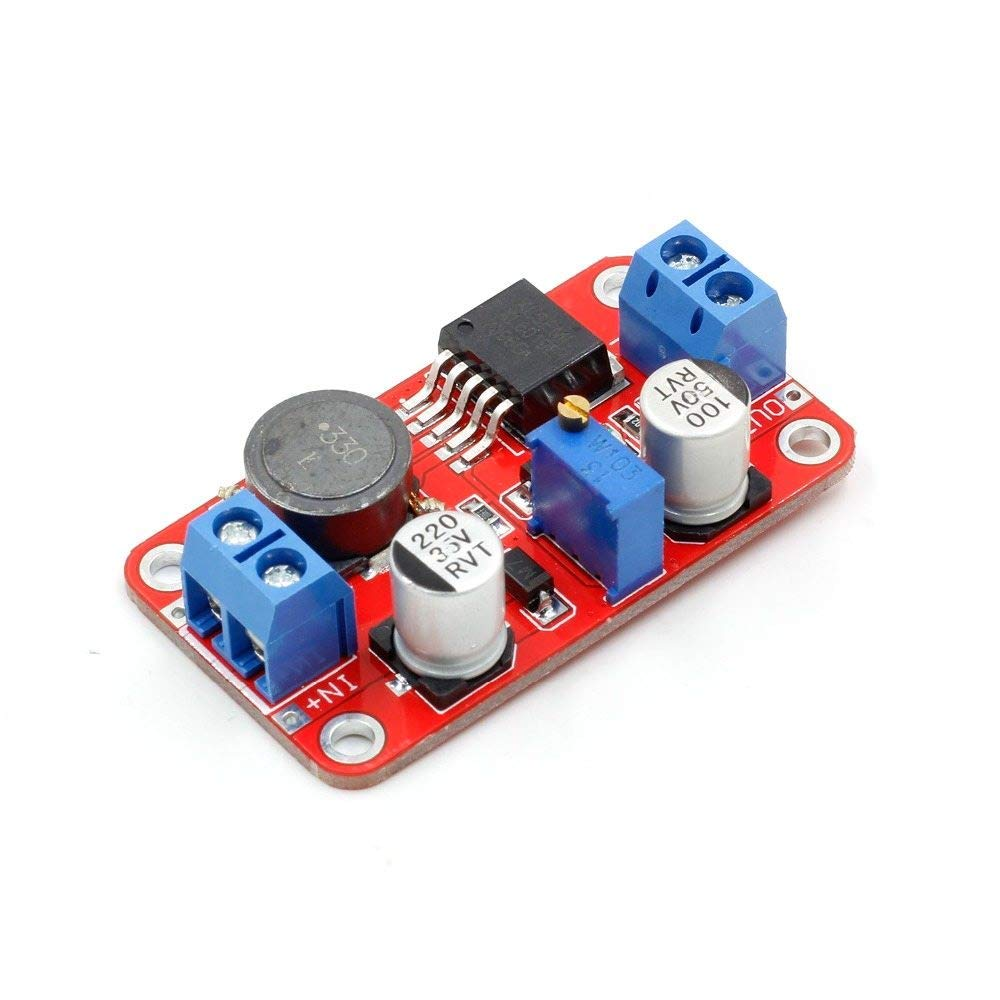
\includegraphics[width=0.45\textwidth]{pics/SP_15.jpg}
    \caption{Módulo elevador de tensión basado en el circuito integrado XL6019,
    fuente: \cite{XL6019Datasheet}.}
    \label{fig:xl6019_boost}
\end{figure}

\section{Integración de los subsistemas}

La integración y conexión de todos los subsistemas descritos anteriormente se
muestra en el diagrama de bloques de la Figura~\ref{fig:bloques_solucion_propuesta}.

\begin{figure}[H]
    \centering
    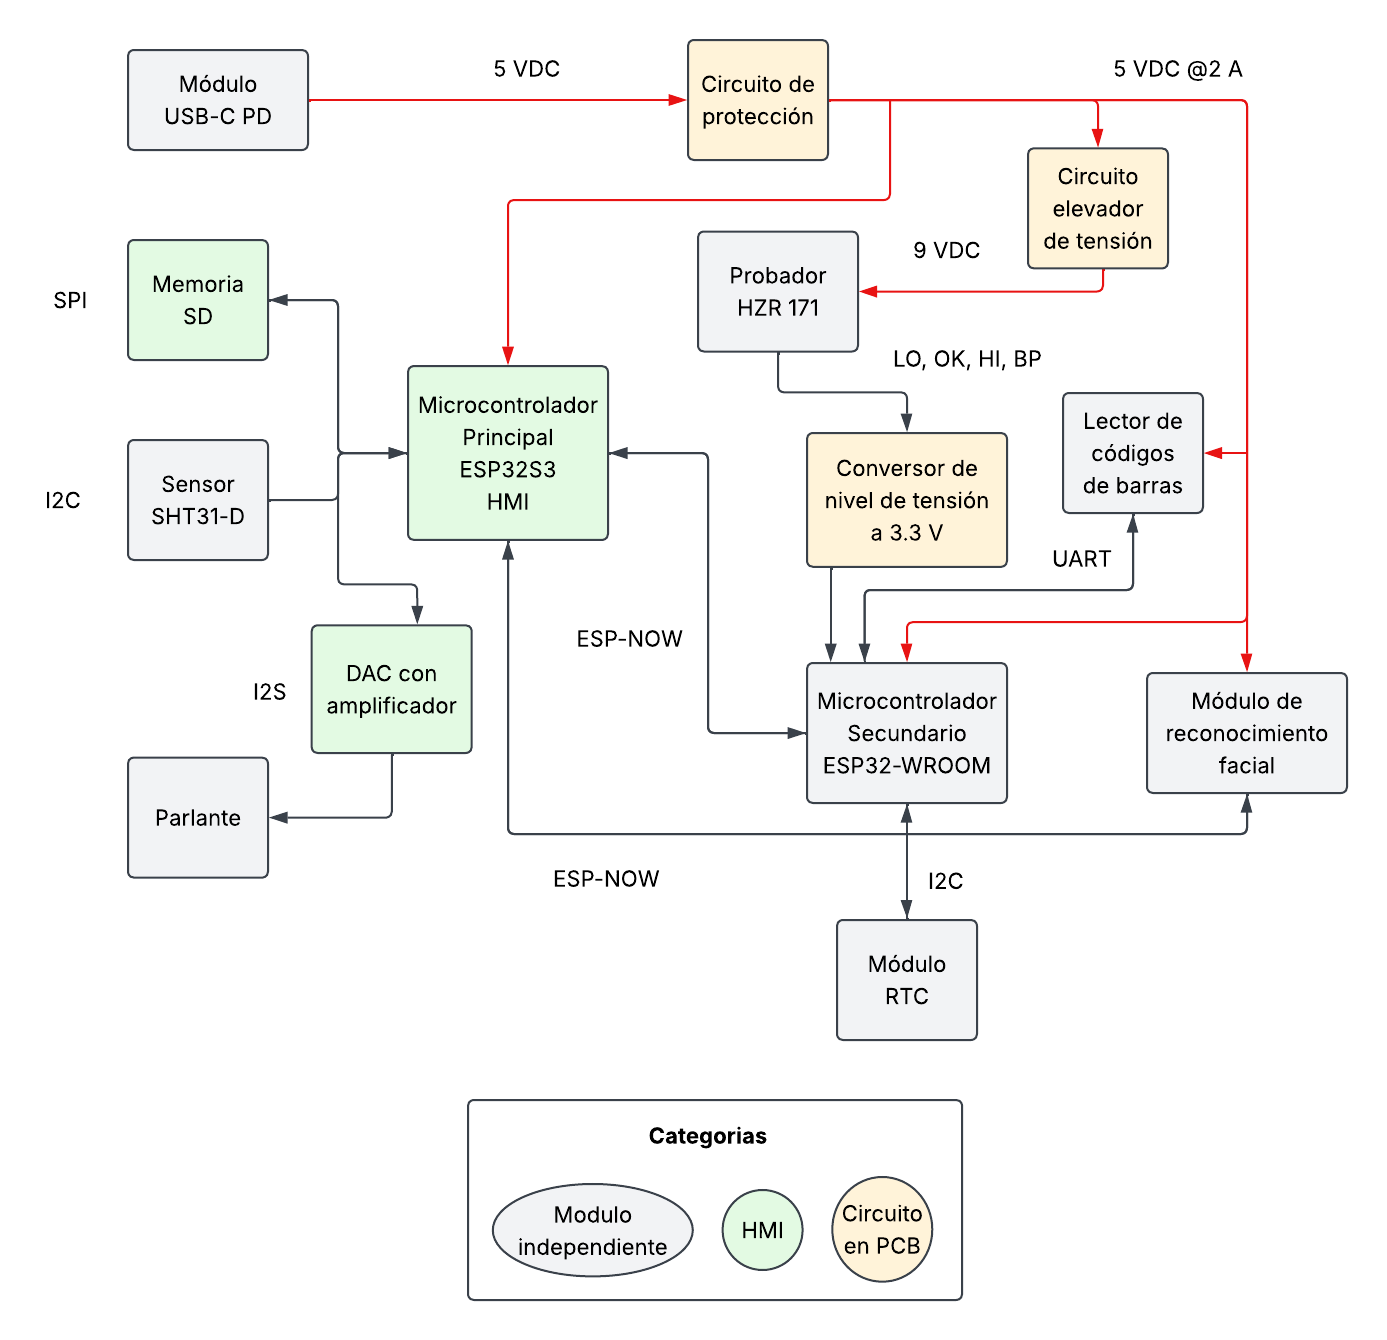
\includegraphics[width=0.95\textwidth]{pics/SP_16.png}
    \caption{Diagrama de bloques de la solución propuesta, fuente:
    elaboración propia.}
    \label{fig:bloques_solucion_propuesta}
\end{figure}

Como se observa en la Figura~\ref{fig:bloques_solucion_propuesta}, las interfaces
se seleccionaron de acuerdo con las características de cada subsistema. El
ESP32-WROOM recibe mediante GPIO las señales del probador HZR 171 y se comunica
con el lector GM67 mediante UART. Por su parte, el sensor ambiental y la memoria
microSD se conectan al controlador principal mediante I2C y SPI,
respectivamente. La comunicación entre los microcontroladores se realiza
mediante ESP-NOW. A su vez un punto a destacar es que la señal $BP$ significa 
button pressed, es decir, que el usuario presionó el botón del probador HZR 171 para iniciar la prueba.

La transferencia de datos propuesta se detalla en la
Figura~\ref{fig:transferencia_datos_microcontroladores}. El controlador principal
coordina el ciclo y solicita información a los nodos secundarios. El
ESP32-WROOM informa el código leído, el estado del botón y las señales del
probador; el ESP32-S3 CAM comunica la detección, la identidad estimada y el valor
de similitud. Esta distribución evita transmitir imágenes completas y reduce la
carga del enlace inalámbrico.

\begin{figure}[H]
    \centering
    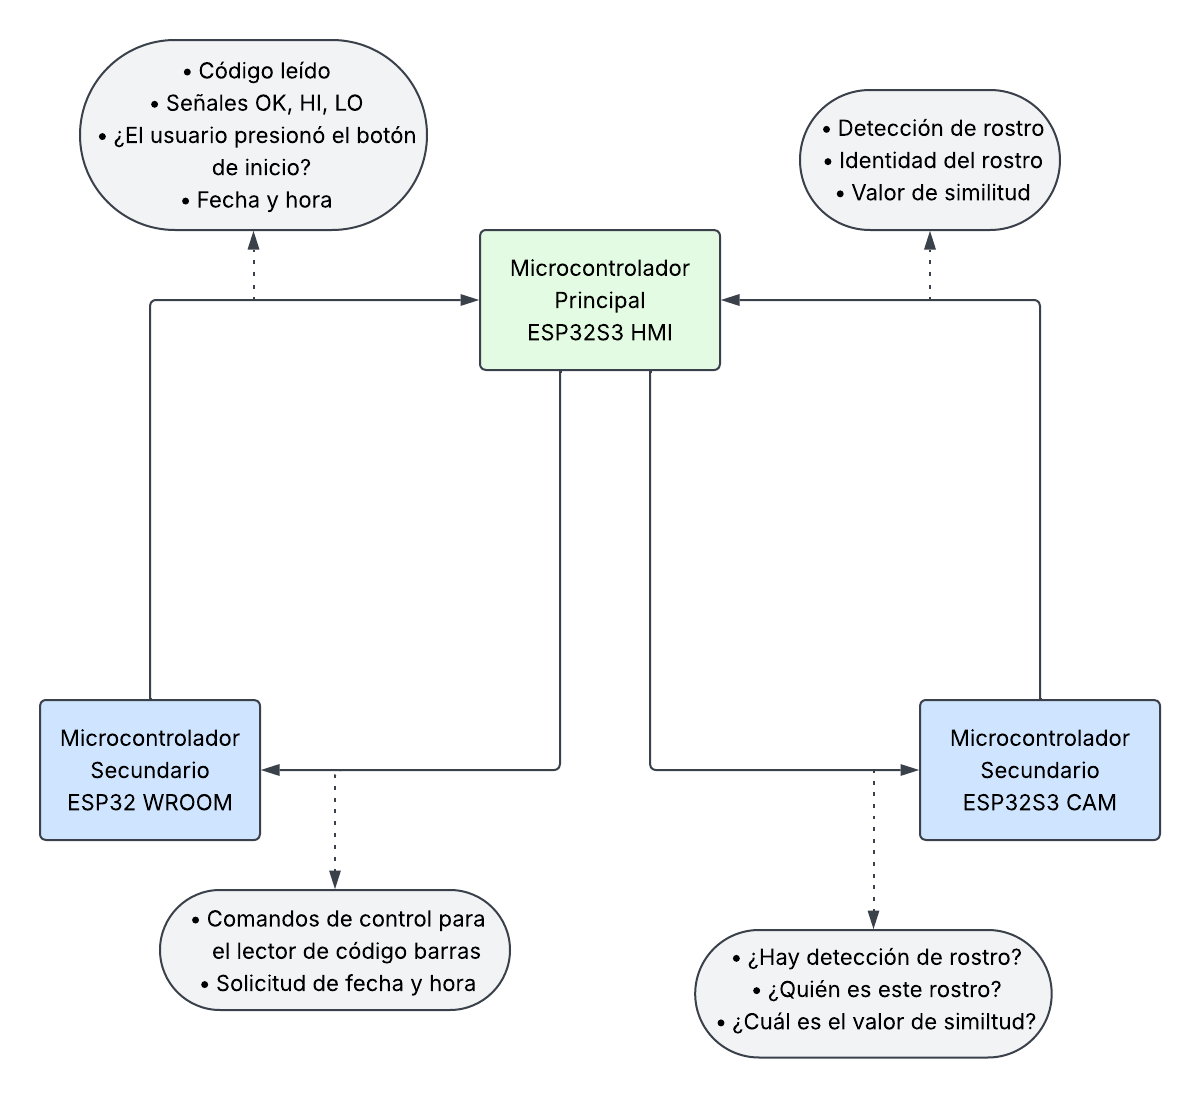
\includegraphics[width=0.80\textwidth]{pics/SP_18.png}
    \caption{Transferencia de datos entre microcontroladores,
    fuente: elaboración propia.}
    \label{fig:transferencia_datos_microcontroladores}
\end{figure}

\section{Integración física}

Para integrar todos los componentes en un único producto se realizará un diseño
CAD utilizando Fusion 360. La estructura física será fabricada mediante
impresión 3D, empleando PLA como material principal. Este diseño permitirá
alojar los diferentes módulos electrónicos, organizar el cableado interno,
facilitar el mantenimiento y mejorar la experiencia de uso del sistema.

El diseño mecánico considerará la ubicación frontal de la pantalla táctil, el
módulo de cámara, el punto de conexión de la pulsera antiestática y los
elementos necesarios para fijar el prototipo en una superficie de trabajo o
pared. Además, se procurará mantener una distribución compacta que facilite su
instalación en laboratorios de electrónica.

\begin{figure}[H]
    \centering
    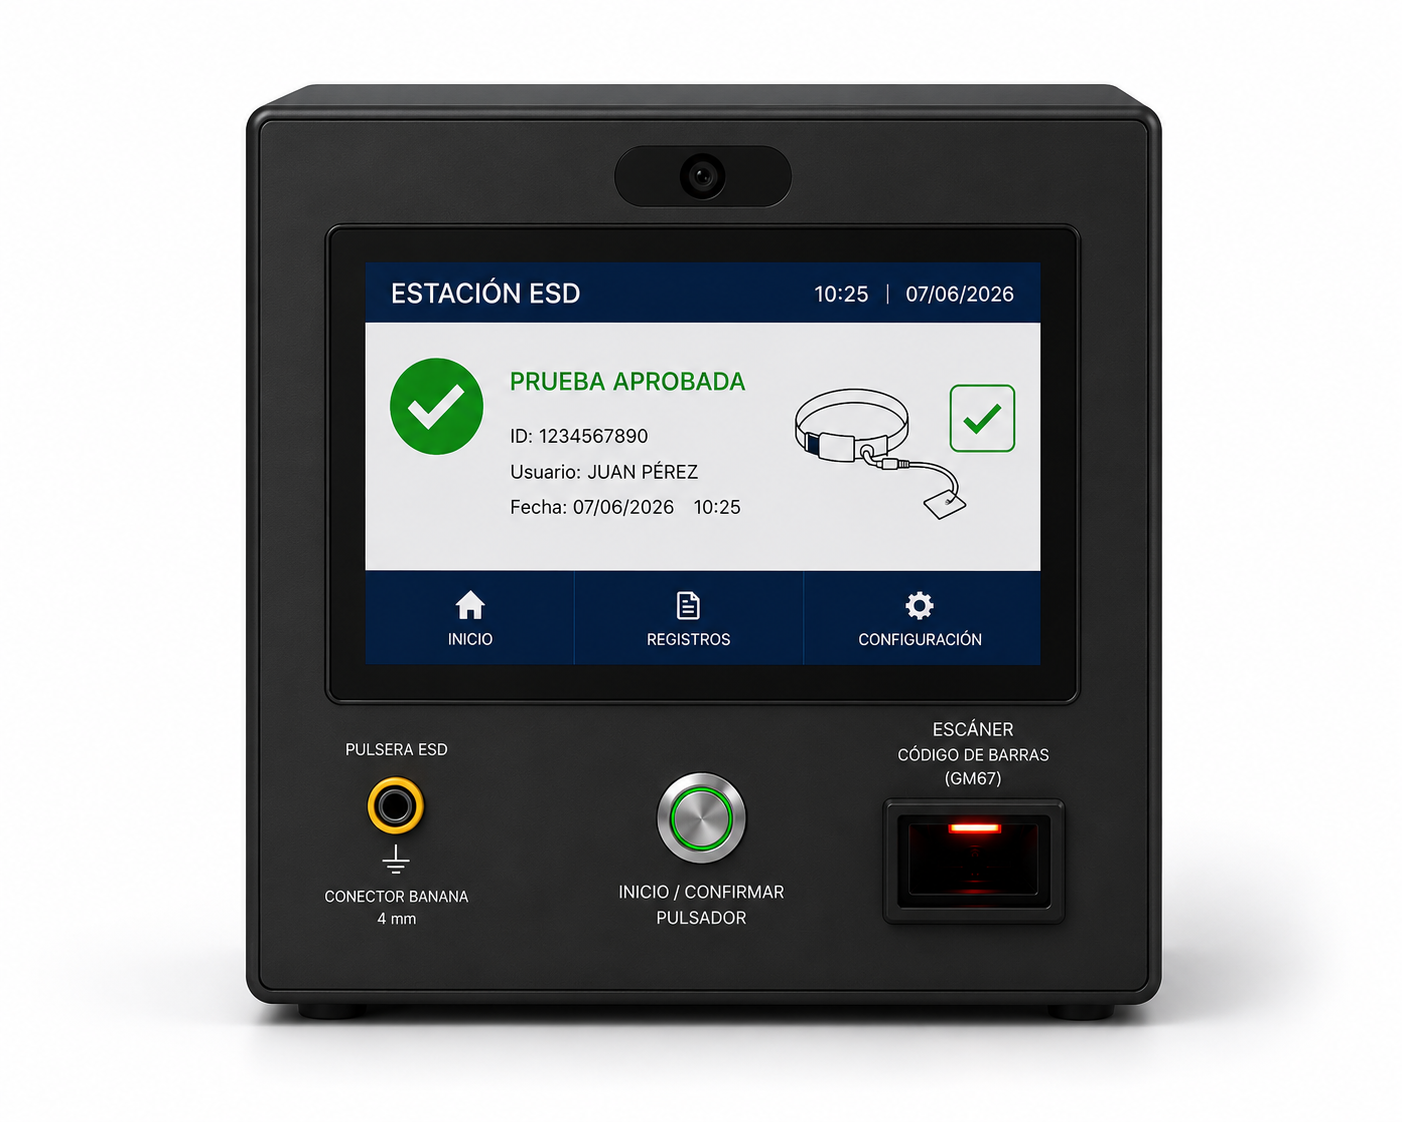
\includegraphics[width=0.75\textwidth]{pics/SP_20.png}
    \caption{Ejemplo conceptual del diseño CAD propuesto para el prototipo,
    fuente: elaboración propia.}
    \label{fig:diseno_cad_propuesto}
\end{figure}

La Figura~\ref{fig:diseno_cad_propuesto} muestra un ejemplo conceptual del
prototipo entregable propuesto. El diseño final podrá variar durante la etapa de
implementación como resultado de consideraciones mecánicas, eléctricas o de
manufactura identificadas durante el desarrollo del proyecto.

\section{Requisitos del sistema}
\label{sec:requisitos_sistema}

A partir de la arquitectura propuesta y del alcance definido para el prototipo, se establecen
los requisitos funcionales y no funcionales del sistema. Estos requisitos permiten delimitar
las capacidades esperadas del sistema inteligente de control ESD y sirven como base para
la posterior validación del prototipo.

\subsection{Requisitos funcionales}

Los requisitos funcionales describen las acciones principales que debe ejecutar el sistema:

\begin{itemize}
    \item RF1: El sistema deberá identificar al usuario mediante lectura de código de barras.

    \item RF2: El sistema podrá realizar reconocimiento facial como mecanismo complementario de identificación.

    \item RF3: El sistema deberá leer los estados entregados por el probador HZR-171 para determinar el resultado de la prueba ESD.

    \item RF4: El sistema deberá mostrar en la interfaz gráfica las instrucciones de operación, el nombre y el identificador del usuario, el resultado de la prueba ESD, la temperatura y la humedad relativa.

    \item RF5: El sistema deberá incorporar temperatura y humedad relativa como información complementaria de cada registro de prueba.

    \item RF6: El sistema deberá almacenar localmente registros que incluyan el nombre y el identificador del usuario, la fecha, la hora, el resultado ESD y las variables ambientales asociadas.

    \item RF7: El sistema deberá generar reportes históricos en formato CSV que incluyan la información contenida en los registros almacenados.

    \item RF8: El sistema deberá permitir la consulta de registros o reportes mediante la interfaz gráfica.

    \item RF9: El sistema deberá detectar la pérdida de comunicación, la
    ausencia de datos obligatorios y los fallos de escritura sin registrar estos
    eventos como pruebas aprobadas.

    \item RF10: El sistema deberá conservar una referencia de fecha y hora cuando se
    interrumpa la alimentación eléctrica.
\end{itemize}

\subsection{Requisitos no funcionales}

Los requisitos no funcionales describen restricciones, condiciones de operación y criterios
de calidad esperados para el sistema:

\begin{itemize}
    \item RNF1: El costo estimado de materiales del prototipo deberá mantenerse por debajo de USD 350.

    \item RNF2: El sistema deberá operar con almacenamiento local, sin depender de servicios en la nube o bases de datos corporativas.

    \item RNF3: El sistema deberá generar registros completos en al menos el 95\% de los ciclos completos de prueba ejecutados.

    \item RNF4: El reconocimiento facial deberá ser opcional y requerir autorización previa del usuario.

    \item RNF5: Los datos personales utilizados durante la validación deberán almacenarse localmente y presentarse de forma anonimizada o agregada en el informe final.

    \item RNF6: El prototipo deberá limitarse a la verificación de pulseras antiestáticas y no deberá considerarse un sistema certificado de control ESD industrial.

    \item RNF7: La arquitectura del sistema deberá ser modular, de forma que permita modificar o sustituir subsistemas sin rediseñar completamente la estación.

\end{itemize}
